%UCD-2: Testa artefatto

\begin{figure}
\centering
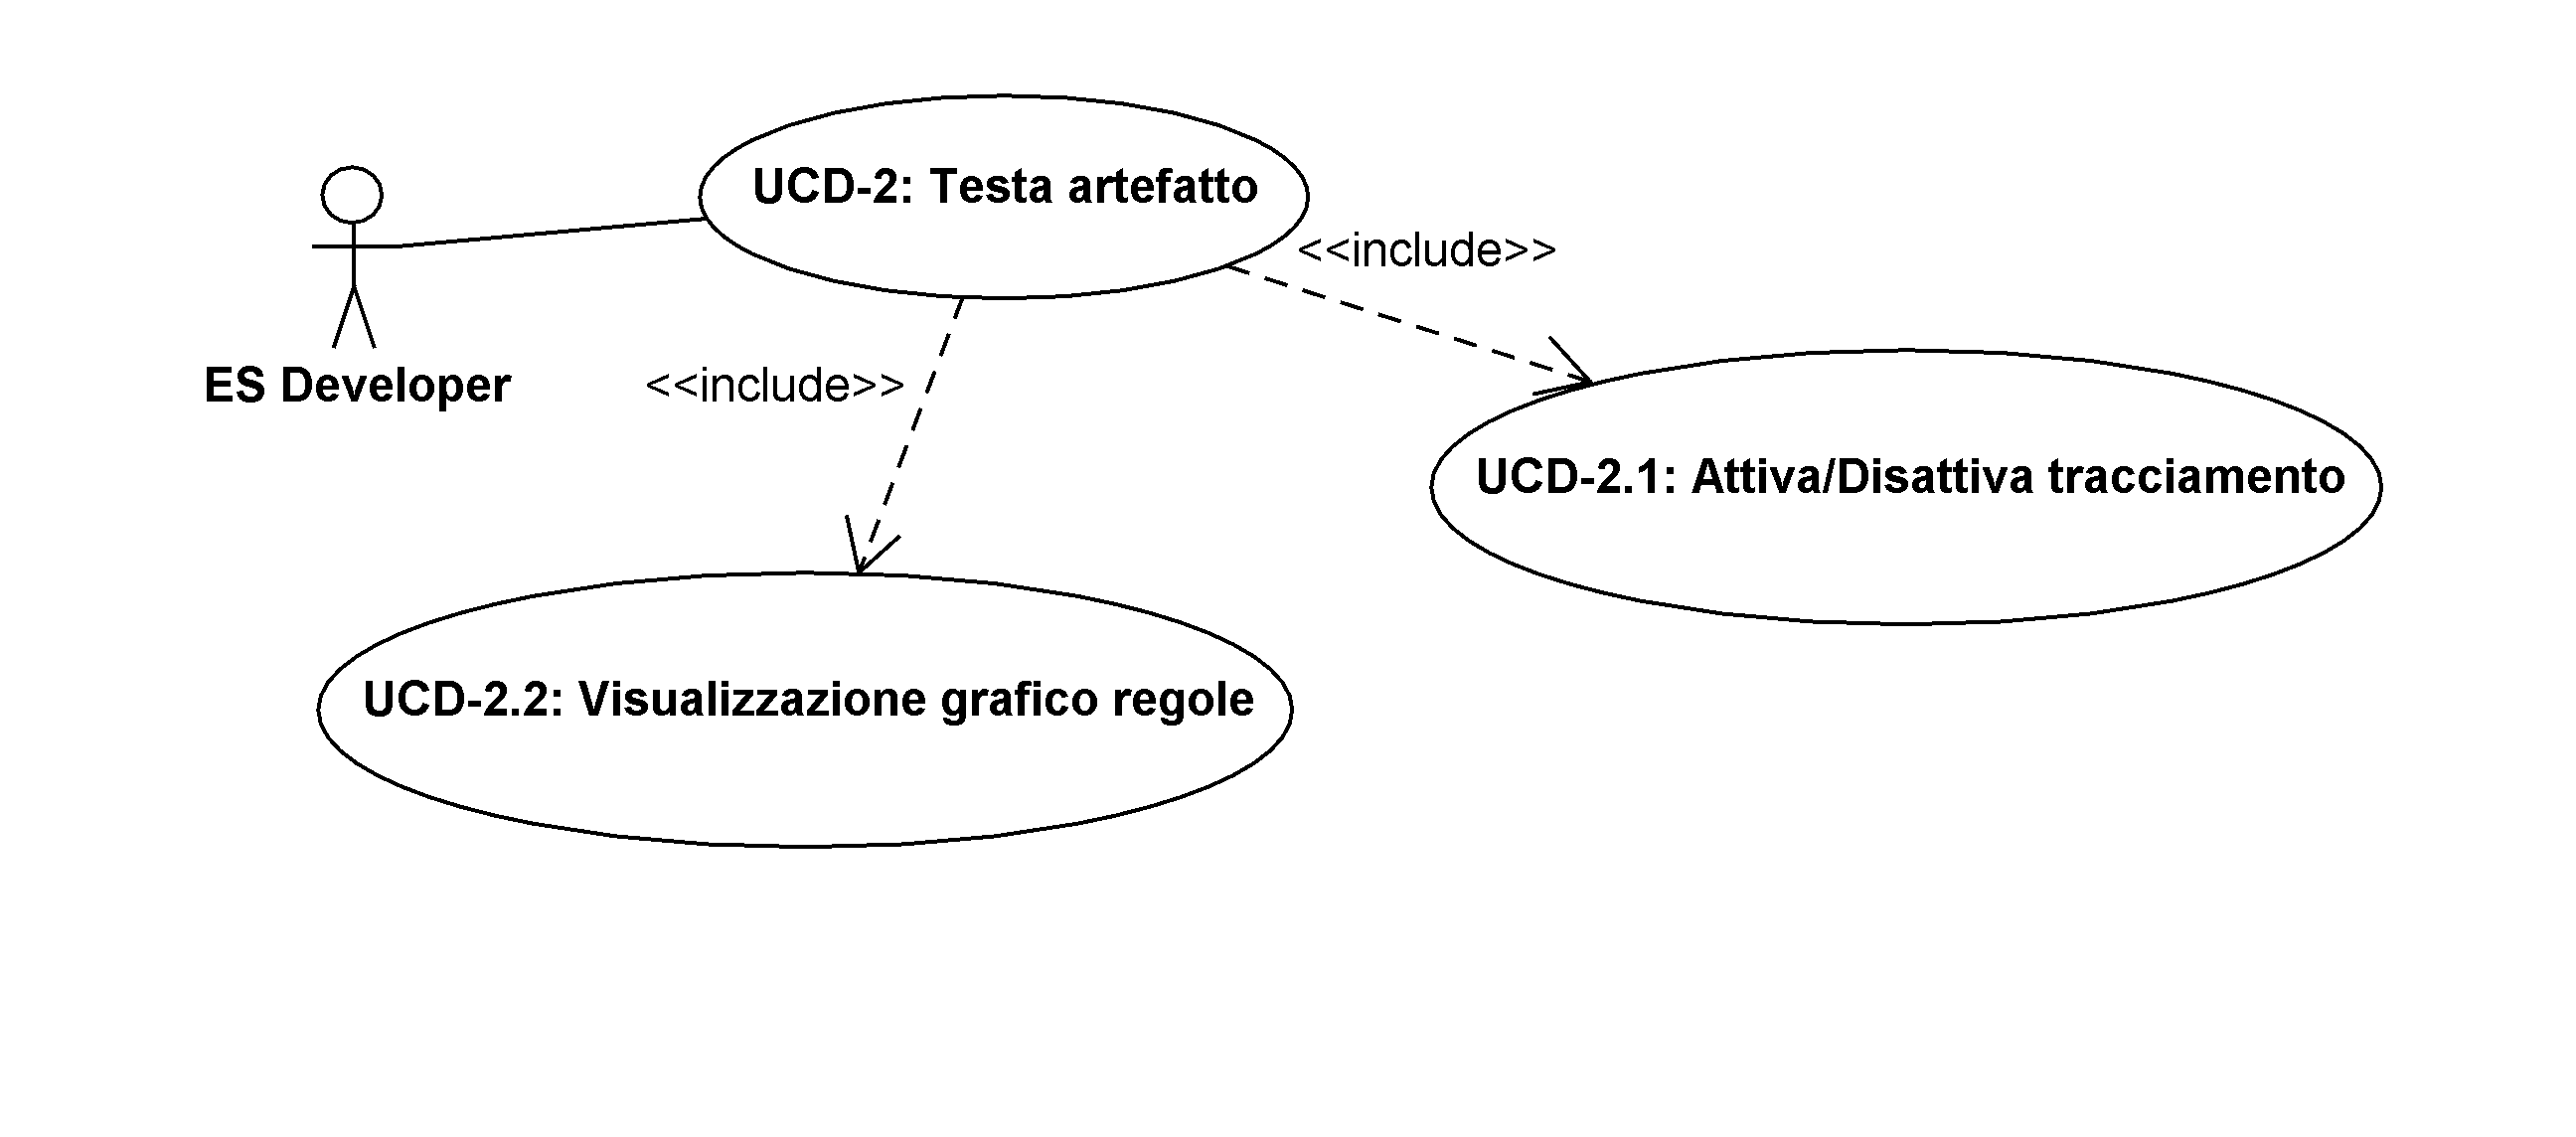
\includegraphics[width=1.1\textwidth]{Immagini/Capitolo2/UseCases/UCD-2.png}
\caption{Diagramma dei casi d'uso UCD-2}\label{fig:uc-ucd-2}
\end{figure}


\begin{itemize}
	\item \textbf{Attori:} ES Developer
	\item \textbf{Scopo e descrizione:} un ES Developer deve essere in grado di testare l'artefatto prodotto valutando un registro del funzionamento dello stesso e le modalità con le quali le definizioni appartenenti all'artefatto vengono interpretate.
	\item \textbf{Pre-condizioni:} l'ES Developer ha realizzato un artefatto, l'artefatto è stato caricato nel sistema. Il sistema attende istruzioni
	\item \textbf{Post-condizioni:} il funzionamento dell'artefatto è stato valutato
	\item \textbf{Flusso principale degli eventi:}
		\begin{enumerate}
			\item l'ES Developer richiede al sistema informazioni per valutare l'artefatto.
			\begin{itemize}
				\item l'ES Developer può richiedere informazioni sull'attività del sistema (si veda caso d'uso \emph{UCD-2.1})
				\item l'ES Developer può richiedere informazioni su come l'artefatto viene interpretato (si veda caso d'uso \emph{UCD-2.2}).
			\end{itemize}
			\item il sistema fornisce le informazioni richieste.
		\end{enumerate}
\end{itemize}


\paragraph{UCD-2.1: Attiva/Disattiva tracciamento}

\begin{figure}
\centering
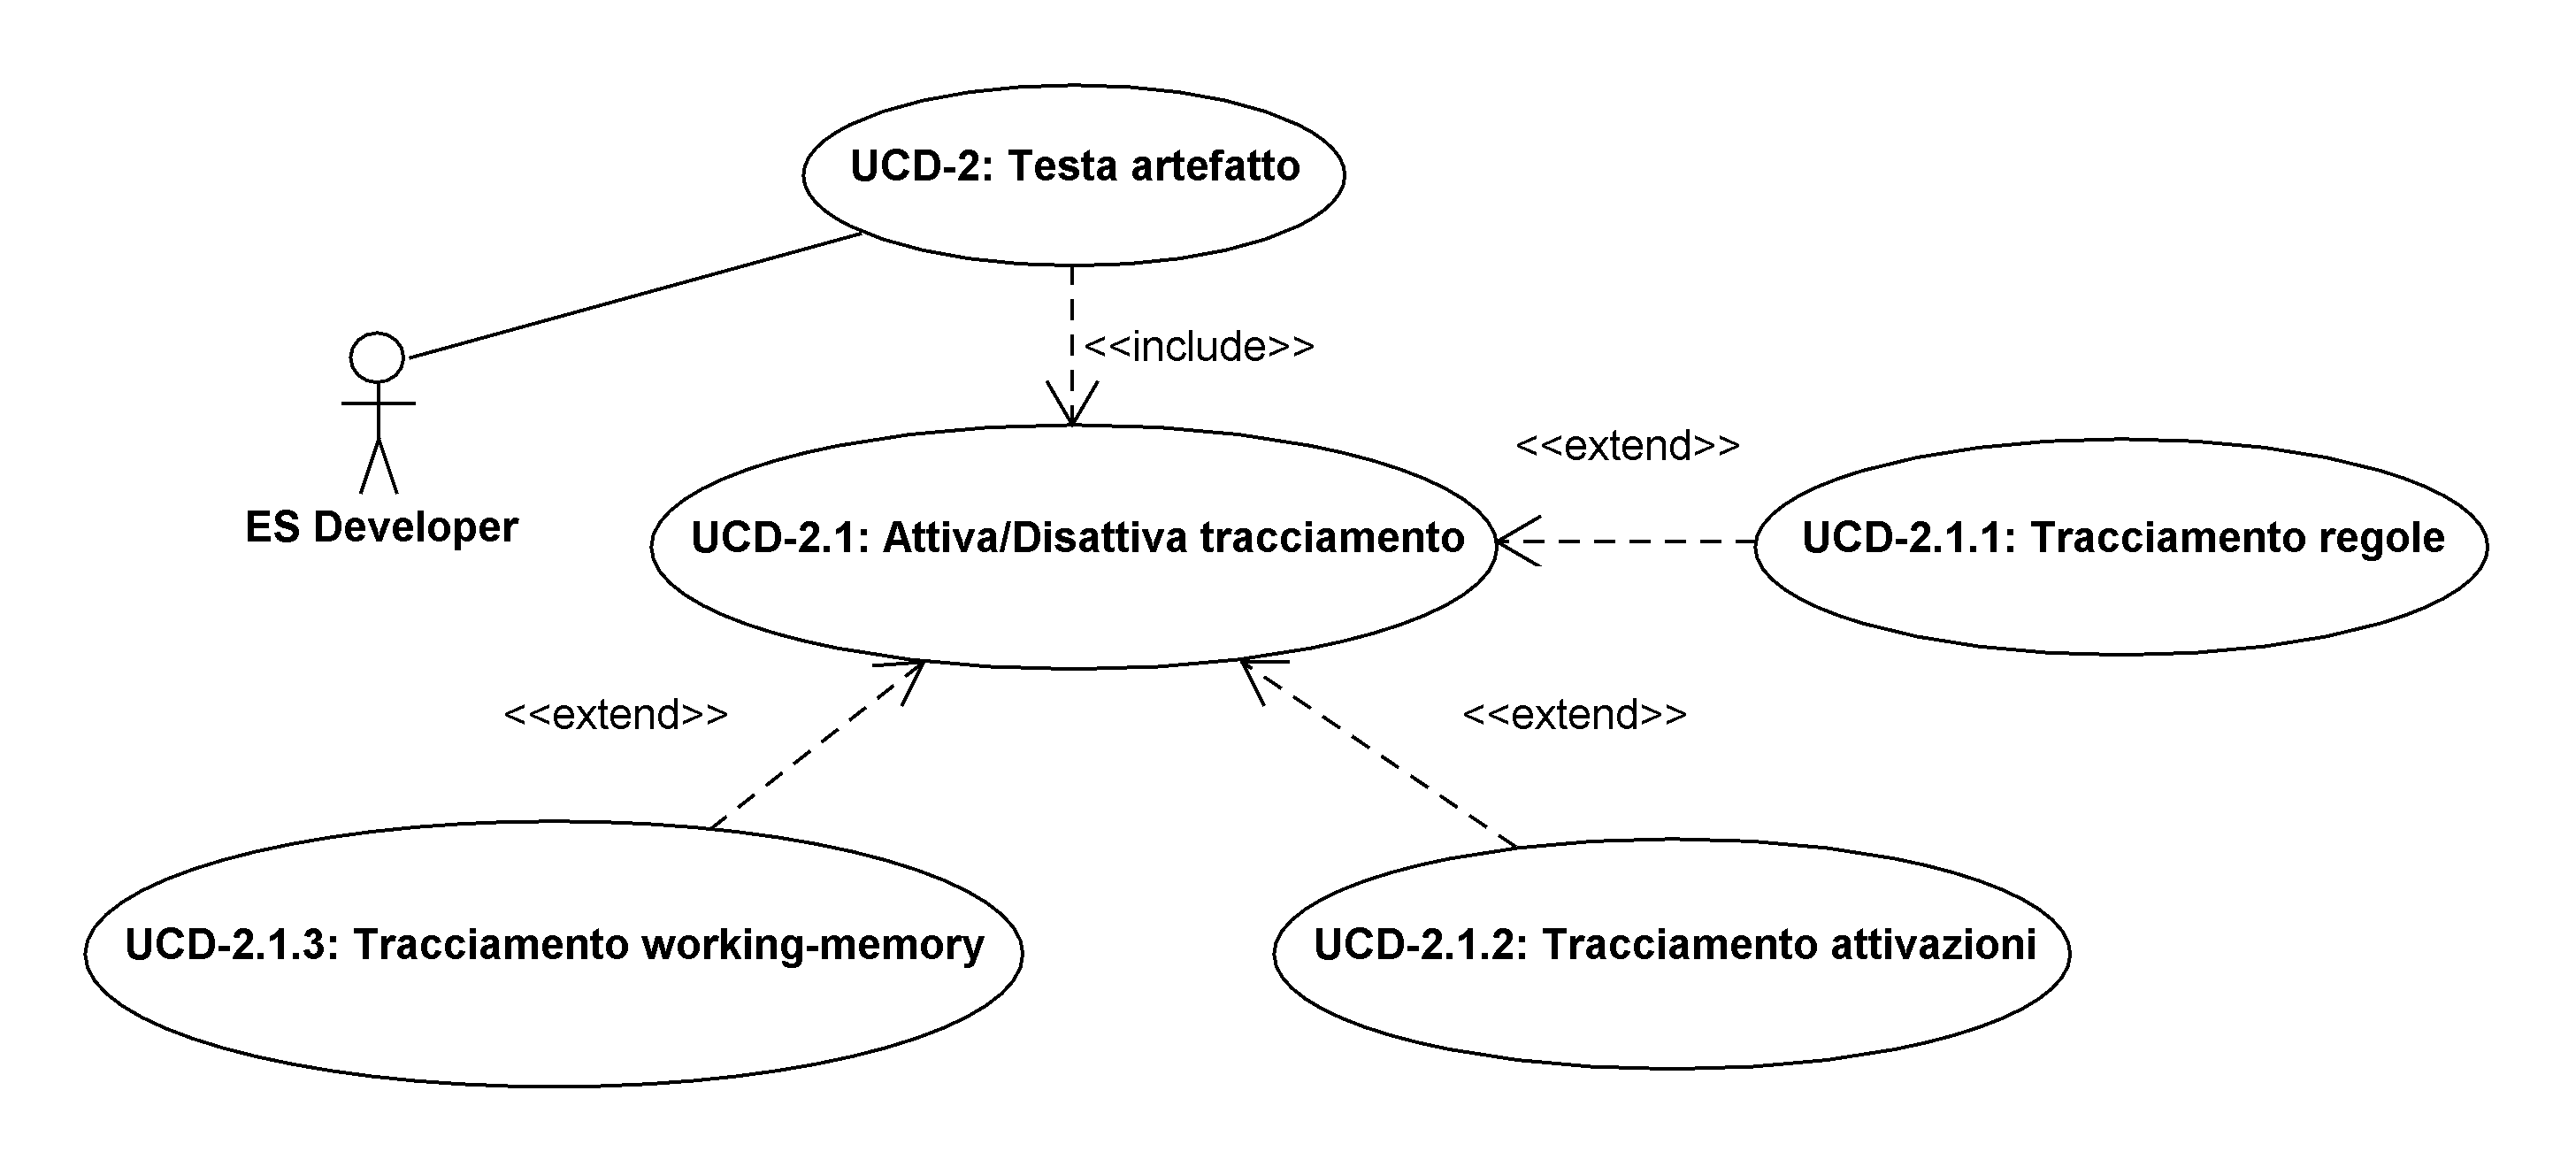
\includegraphics[width=1.1\textwidth]{Immagini/Capitolo2/UseCases/UCD-2_1.png}
\caption{Diagramma dei casi d'uso UCD-2.1}\label{fig:uc-ucd-2.1}
\end{figure}

La descrizione comprende quella dei casi d'uso \emph{UCD-2.1.1}, \emph{UCD-2.1.2}, \emph{UCD-2.1.3} in quanto identici, a meno del tipo di informazioni che vengono tracciate.

\begin{itemize}
	\item \textbf{Attori:} ES Developer
	\item \textbf{Scopo e descrizione:} un ES Developer deve essere in grado di modificare le impostazioni riguardo al tracciamento di regole, attivazioni e modifiche alla \emph{working-memory}.
	\item \textbf{Pre-condizioni:} ES Developer ha caricato un artefatto nel sistema. Il sistema attende istruzioni
	\item \textbf{Post-condizioni:} le impostazioni di tracciamento risultano modificate
	\item \textbf{Flusso principale degli eventi:}
		\begin{enumerate}
			\item l'ES Developer modifica le impostazioni riguardanti il tracciamento
			\begin{itemize}
				\item l'ES Developer può attivare (risp. disattivare) il tracciamento delle regole eseguite
				\item l'ES Developer può attivare (risp. disattivare) il tracciamento delle attivazioni disponibili
				\item l'ES Developer può attivare (risp. disattivare) il tracciamento delle modifiche alla \emph{working-memory}				
			\end{itemize}
			\item il sistema modifica le impostazioni di tracciamento dell'elemento indicato
		\end{enumerate}
	\item \textbf{Flusso alternativo:}
		\begin{enumerate}
			\item l'ES Developer richiede l'attivazione (risp. disattivazione) di un tracciamento già attivo (risp. non attivo).
			\item il sistema ignora la richiesta
		\end{enumerate}
\end{itemize}


\paragraph{UCD-2.2: Visualizzazione grafico regole}

\begin{itemize}
	\item \textbf{Attori:} ES Developer
	\item \textbf{Scopo e descrizione:} un ES Developer deve essere in grado di richiedere informazioni riguardanti le modalità con le quali il sistema interpreta una regola.
	\item \textbf{Pre-condizioni:} ES Developer ha caricato un artefatto nel sistema. Il sistema attende istruzioni
	\item \textbf{Post-condizioni:} Il sistema attende istruzioni
	\item \textbf{Flusso principale degli eventi:}
		\begin{enumerate}
			\item l'ES Developer richiede informazioni riguardanti l'interpretazione di una regola
			\begin{itemize}
				\item l'ES Developer può indicare una regola specificandone il nome
				\item l'ES Developer può indicare un insieme di regole specificandone i nomi
			\end{itemize}
			\item il sistema fornisce le informazioni richieste
		\end{enumerate}
	\item \textbf{Flusso alternativo \#1:}
		\begin{enumerate}
			\item l'ES Developer specifica un nome di regola non valido
			\item il sistema ignora la richiesta, notificando l'errore
		\end{enumerate}
	\item \textbf{Flusso alternativo \#2:}
		\begin{enumerate}
			\item l'ES Developer inserisce un nome non valido specificando un insieme di regole
			\item il sistema ignora la richiesta, notificando l'errore
		\end{enumerate}
\end{itemize}

